\chapter{Software}
\label{cha:software}

Oprogramowanie słuchawek zostało napisane w języku C z wykorzystaniem bibliotek HAL, które zawierają dużo gotowych funkcji, na przykład do uruchomienia timera lub do odczytu wartości z przetwornika. Użyto narzędzia \textit{System Workbench for STM32}, które jest zbudowane na popularnym IDE \textit{Eclipse}. Kod do konfiguracji i inicjalizacji peryferiów został wygenerowany z użyciem \textit{CubeMX}. Dodatkowo jako program pomocniczy zainstalowano STMStudio, które korzysta z \textit{ST LINKa} do odczytu przez USB wartości adresów w pamięci procesora (zmiennych) i wyświetla je w formie wykresu lub tabeli.

Tak jak przy pozostałych elementach projektu, wykorzystano repozytorium do zapisywania postępów: \url{https://github.com/Hoplophile/TacticalHeadphones_SW.git}

\begin{figure}[H]
	\centering
	\begin{subfigure}{.48\textwidth}
		\centering
		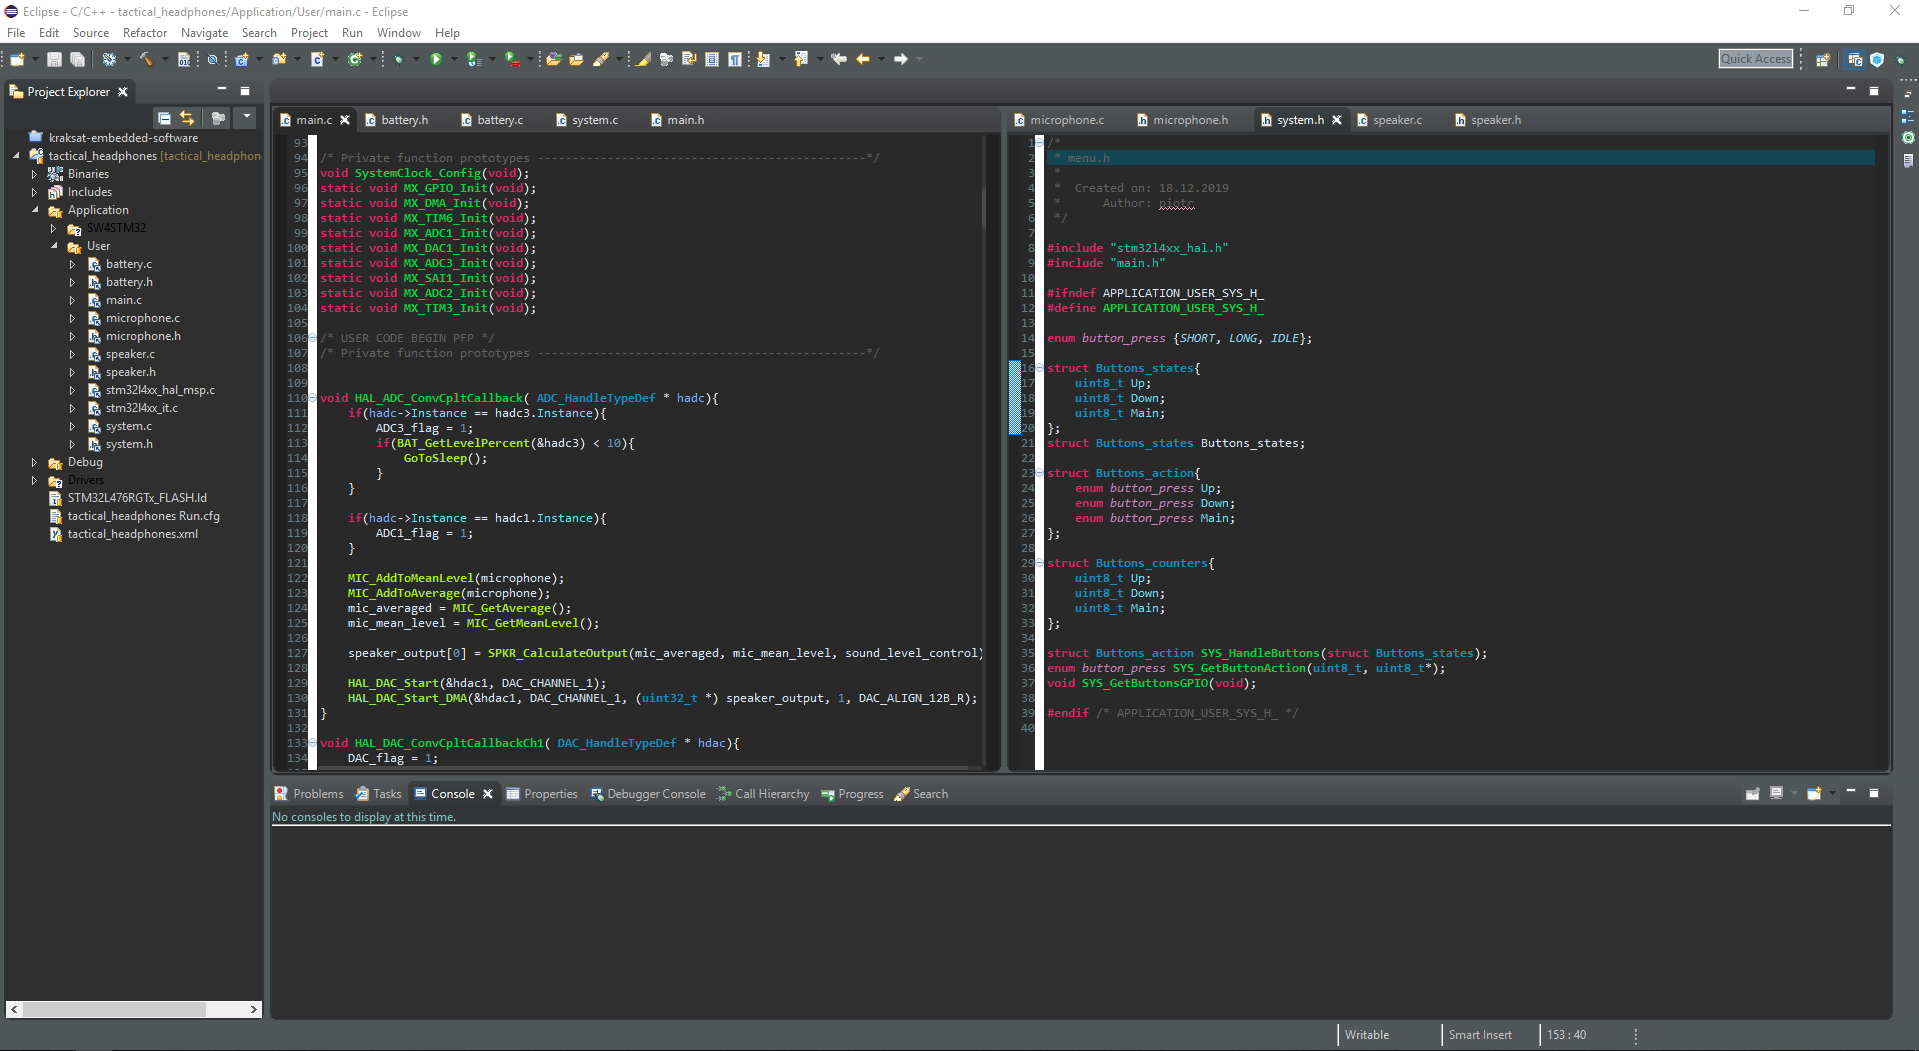
\includegraphics[height=4.2cm]{zdjecia/eclipse.png}
		\subcaption{System Workbench for STM32}
	\end{subfigure}
	\begin{subfigure}{.48\textwidth}
		\centering
		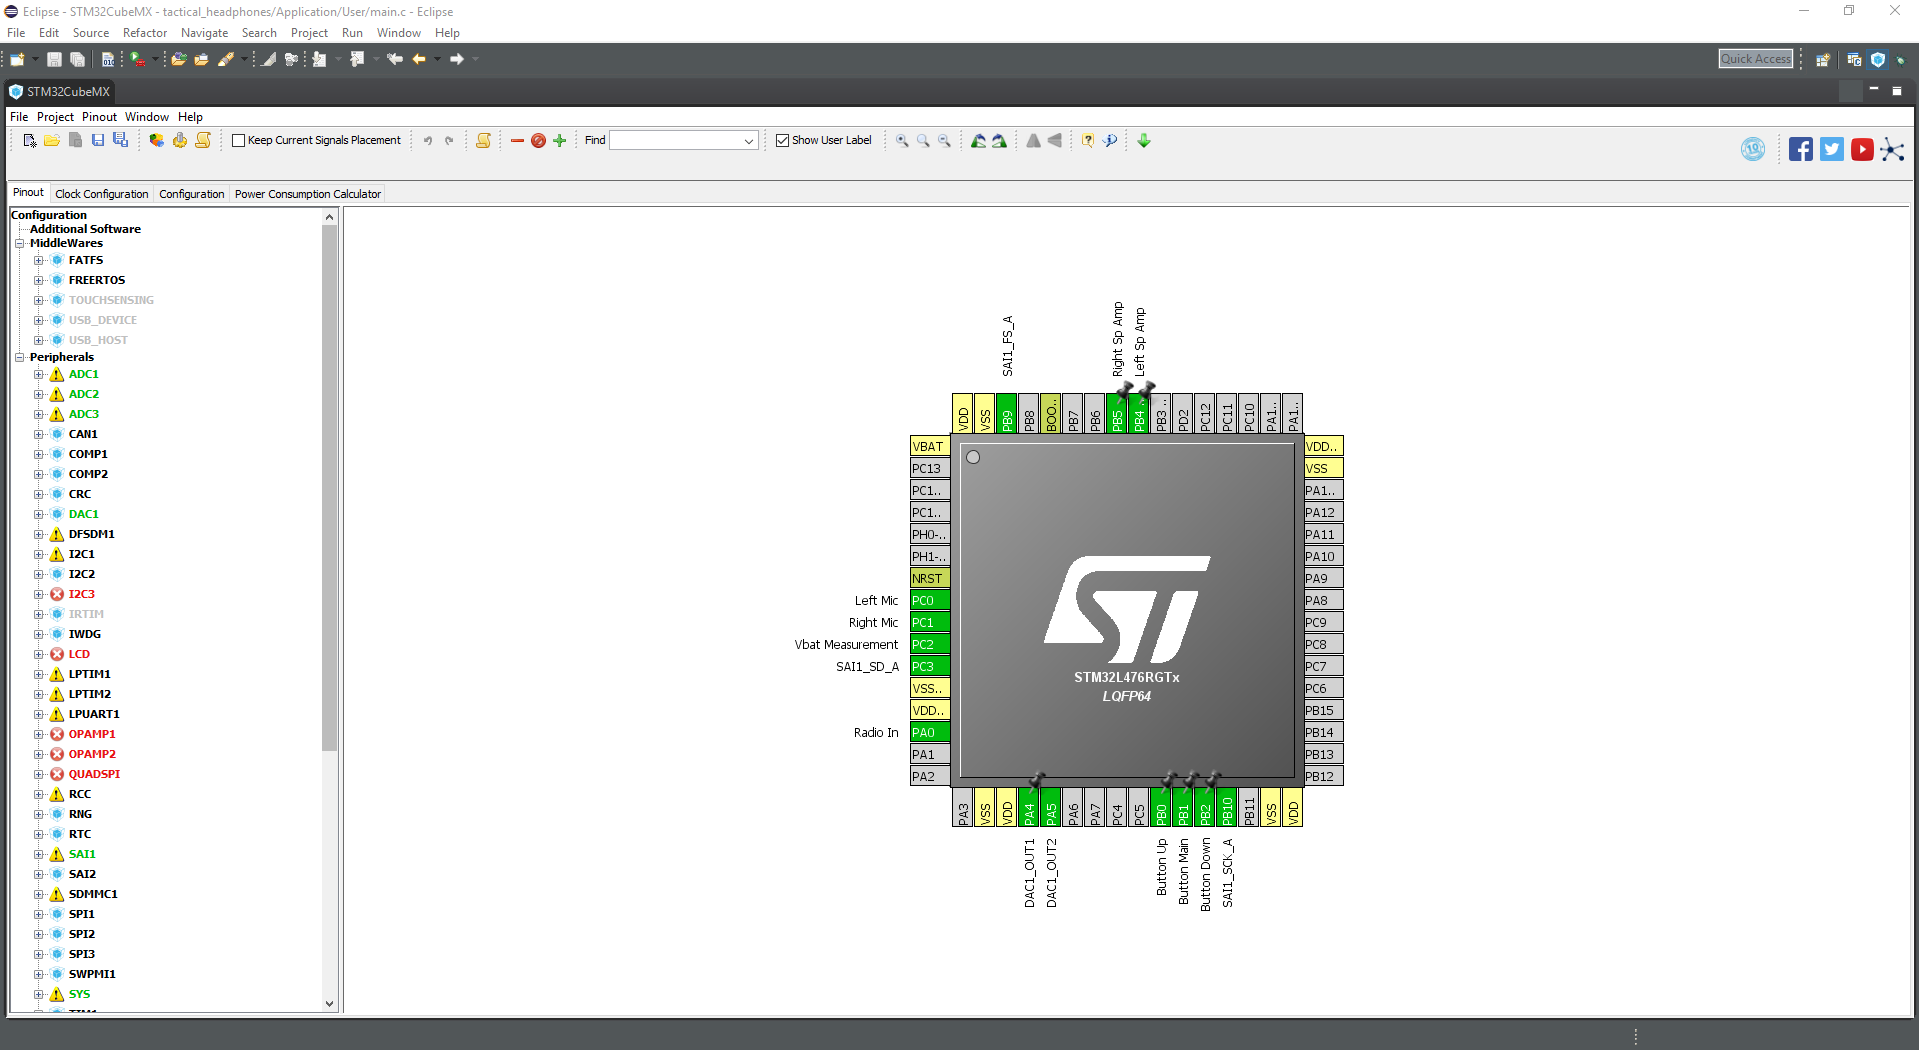
\includegraphics[height=4.2cm]{zdjecia/cubemx.png}
		\subcaption{CubeMX}
	\end{subfigure}
	\begin{subfigure}{.48\textwidth}
		\centering
		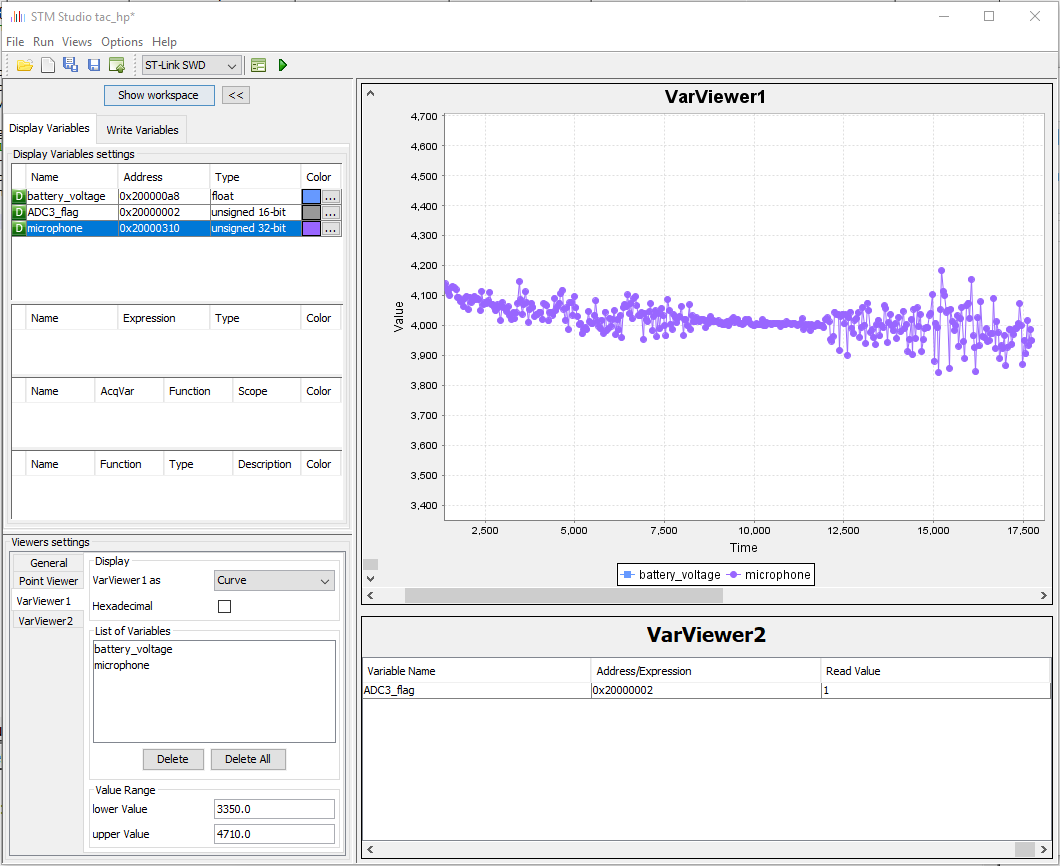
\includegraphics[height=4.2cm]{zdjecia/stmstudio.png}
		\subcaption{STMStudio}
	\end{subfigure}
	\caption{\label{pic:IDE} Narzędzia użyte do rozwoju oprogramowania}
\end{figure}

Kod był pisany tak, aby rozdzielić program na funkcje wykonujące niewielkie fragmenty. Przewidziano także elastyczną możliwość modyfikacji lub dodawania funkcjonalności, na przykład implementując do $V_{BAT}$ 3 funkcje, odczytujące: wartość surową oraz bazujące na niej wartości w Voltach i procentach. W obecnej wersji użyta została ta ostatnia.

Dla lepszej nawigacji, zastosowano konwencję nazewnictwa funkcji - <SKRÓTOWA\_NAZWA\_PLIKU>\_<funkcjonalnośćFunkcji>. Na przykład funkcja dodająca wartość do średniego poziomu sygnału mikrofonu zawarta w pliku \textit{microphone.c} została nazwana \textit{MIC\_AddToMeanLevel}.

Każda funkcja ma przed definicją krótki opis funkcjonalności oraz przyjmowanych i zwracanych wartości.

Do wszystkich zadań użyto przerwań, aby zmaksymalizować wydajność obliczeniową i nie blokować procesów. Pętla główna programu jest pusta.

\section{System słuchawek}
\label{cha:soft_sys}

Funkcje związane ze sterowaniem słuchawkami znajdują się w pliku \textit{system.c}. Zaimplementowano funkcje do odczytu krótkich ($\textless 300ms$) i długich ($\textgreater 3s$) przyciśnięć wszystkich 3 przycisków dostępnych dla użytkownika. Stany zapisywane są do struktury z 3 polami typu \textit{enum}, przyjmującymi wartości \textit{IDLE}, \textit{LONG}, \textit{SHORT}. Sprawdzanie jest wyzwalane przez timer co $30ms$. Mimo, że w obecnej wersji wykorzystywane są tylko krótkie przyciśnięcia przycisków \textbf{plus} i \textbf{minus} do podgłaśniania i przyciszania dźwięku w trybie \textbf{NORMAL} oraz przytrzymanie głównego do usypiania/wybudzania systemu, to w myśl elastyczności modyfikacji, stan wszystkich przycisków jest monitorowany w ten sam sposób. Dodatkowym efektem przycisku mogłoby być odtworzenie krótkiego dźwięku, sygnalizującego jego przyciśnięcie. Nie zaimplementowano jednak tej funkcji.

Działanie słuchawek opiera się na przełączaniu między trzema stanami:

\begin{itemize}
	\item \textbf{NORMAL} - słuchawki mają bezpośrednio przekazywać dźwięk z zewnątrz i są nastawione na jakość sygnału. Jest to domyślny tryb, do którego system przechodzi po wybudzeniu przez użytkownika przytrzymaniem głównego przycisku.
	
	\item \textbf{CANCELLING} - próbki odbierane przez mikrofon muszą zostać jak najszybciej dodane do kolejki, skąd ze ściśle określonym opóźnieniem (równym czasowi przelotu fali akustycznej) zostają wypuszczone do głośnika. Warunkiem przejścia do tego trybu jest zmierzenie w stanie \textbf{NORMAL} amplitudy wykraczającej poza określony próg. System wraca do \textbf{NORMAL}, jeśli amplituda ponownie spadnie poniżej progu.
	
	\item \textbf{SLEEP} - tryb oszczędzania baterii, w którym wyłączone są przerwania od wszystkich przetworników oraz za pomocą pinów GPIO wzmacniacze głośników\ref{cha:glosniki}. Przejście do tego stanu może być wywołane przez zanotowanie poziomu baterii poniżej $3,12V$ ($10\%$) lub przez przytrzymanie głównego przycisku przez $3s$.
\end{itemize}

Odczyt poziomu naładowania akumulatora został wydzielony do pliku \textit{battery.c}. Tak jak zostało to opisane na początku tego rozdziału, $V_{BAT}$ można pobrać w trzech różnych formach. Odczyt jest wykonywany na zakończenie konwersji, tak samo jak w przypadku mikrofonu \ref{cha:soft_mic}, lecz wykorzystano dodatkowo \textit{clock prescaler} o wartości $256$ (największej możliwej). Sprawdzanie napięcia na baterii nie wymaga dużej częstotliwości, a jej zmniejszenie umożliwia pozostałym funkcjonalnościom nieprzerwane działanie.

\section{Odczyt sygnału z mikrofonu}
\label{cha:soft_mic}

Pierwsze kroki z oprogramowaniem słuchawek polegały na inicjalizacji peryferiów potrzebnych do odczytu analogowego wyjścia mikrofonu. Od początku wybrano odczyt ADC z użyciem DMA (ang. \textit{Direct Memory Access} - Bezpośredni Dostęp do Pamięci). Jest to podejście, w którym przetwornik, za pomocą kontrolera DMA, ma bezpośredni dostęp do pamięci RAM. Dzięki temu główny procesor zostaje odciążony od przesyłania danych i może w tym czasie wykonywać inne operacje. Odczyt z przetworników wykonywano w ciele funkcji \textit{HAL\_ADC\_ConvCpltCallback}, która jest wywoływana automatycznie po zakończonej konwersji ADC w trybie przerwań.

Czas konwersji wbudowanego, 12-bitowego przetwornika wynosi zgodnie ze specyfikacja mikrokontrolera $t_s$ (sampling time) + $12,5$ cykli zegara\cite{STM32L4}. Przy taktowaniu $48MHz$ jeden cykl trwa $0,208ns$, a $t_s$ jest ustawiony na $2,5$, więc czas konwersji wynosi $0,313 \mu s$.

Funkcje związane z odczytem i bezpośrednim przetwarzaniem danych z mikrofonów znajdują się w pliku \textit{microphone.c}.

\textbf{OPISAĆ MIKROFON CYFROWY, USREDNIANIE I FIR}


\section{Minimalizacja szumów}
\label{cha:soft_noise}

Począkowo użyto zegara HSI (ang. \textit{High Speed Internal} - Wysokiej Prędkości Wewnętrzny [zegar]) do wyzwalania przetwornika ADC. Jego podstawowa częstotliwość wynosi $16MHz$. Z wykorzystaniem wbudowanego PLLa zwiększono prędkość do $80MHz$ i użyto jako źródło dla całego mikrokontrolera razem z peryferiami. W trakcie rozwoju oprogramowania okazało się, że odczyt jest bardzo zaszumiony, dlatego zrezygnowano z użycia PLLa, który był potencjalnym źródłem szumu. Podstawowa częstotliwość HSI była jednak za mała, więc zmieniono źródło na MSI (ang. \textit{Multi Speed Internal} - Wielo-Prędkościowy Wewnętrzny [zegar]), którego częstotliwość podstawowa wynosi $48MHz$ i taka została ostatecznie użyta w całym systemie.

\begin{figure}[H]
	\centering
	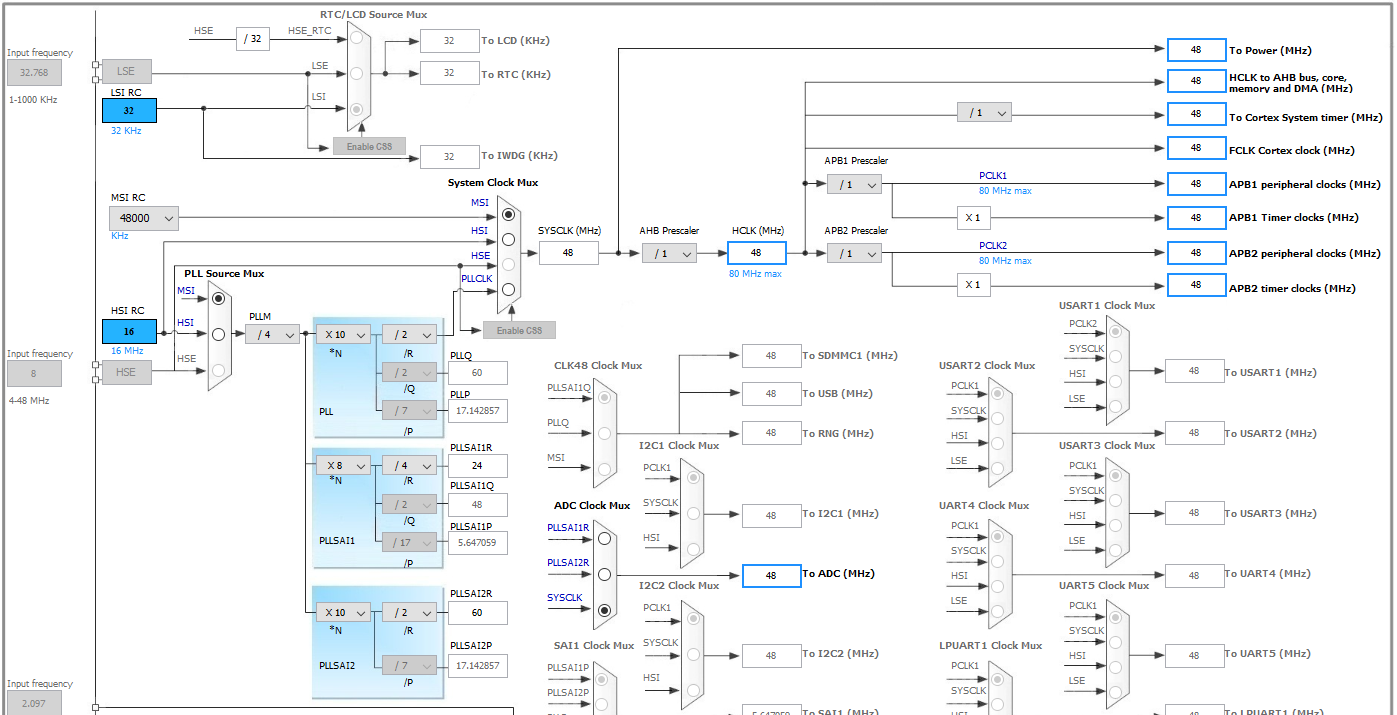
\includegraphics[scale=0.4]{zdjecia/clocks.png}
	\caption{\label{pic:clocks}Konfiguracja zegarów mikrokontrolera w \textit{CubeMX}}
\end{figure}

Kolejnym zabiegiem mającym polepszyć jakość odczytywanego sygnału było zatrzymywanie przetwarzania ADC w trakcie pracy DAC i odwrotnie. Negatywnym skutkiem było spowolnienie systemu, jednak wysoka jakość jest potrzebna głównie w trybie przekazywania dźwięków z otoczenia do użytkownika. Gdyby więc okazało się, że system nie nadąża z nakładaniem antyfazy w celu wyciszania - na potrzeby zwiększonej szybkości, a kosztem jakości, system mógłby przejść w tryb jednoczesnego przetwarzania ADC i DAC.

\textbf{OVERSAMPLING}

\section{Wysyłanie sygnału do głośnika}
\label{cha:soft_spkr}

Do sterowania głośnikami wykorzystano wbudowane przetworniki DAC i tak jak przy mikrofonach - użyto DMA oraz wywołania funkcji \textit{HAL\_DAC\_ConvCpltCallback}. Sygnał z mikrofonu jest wcześniej sprowadzany do wartości AC (bez składowej stałej). Z tego powodu wyjścia przetworników są obliczane w funkcji \textit{SPKR\_CalculateOutput} poprzez przesunięcie go o 2048, czyli do połowy maksymalnej wartości DAC (12-bitowego) i mnożone przez przekazany parametr głośności. 

Nie udało się zaprogramować do końca sterowania głośnością, jednak istotnym jest, aby maksymalna wartość iloczynu parametru sterującego i sygnału z mikrofonu nie wykroczyły poza połowę wartości DAC (2047). Zgodnie ze opisem specyfikacji w rozdziale \ref{cha:mikrofony} o mikrofonach, maksymalna zmiana sygnału wyjściowego wynosi $447,75 mV$. W 12-bitowym przetworniku ADC z napięciem referencyjnym $3,3V$ jeden bit odpowiada $0,81mV$, więc odczyt nie powinien przekroczyć wartości $554$. Parametr głośności nie może więc przekroczyć $3,7$. Należałoby wziąć pod uwagę niedokładność pomiaru ADC, jednak faktyczna wartość z pewnością byłaby dużo mniejsza z uwagi na brak potrzeby odtwarzania głośnych dźwięków w słuchawkach.

\textbf{CZAS KONWERSJI DAC, UŻYCIE OPAMPA DO PRZYSPIESZENIA}

\section{Analiza dźwięku i wyciszanie}
\label{cha:soft_analysis}

Na implementację aktywnego dostosowania dźwięku zabrakło czasu. Zgodnie z założeniami trzeba by stale porównywać amplitudę sygnału mikrofonu z określonym poziomem odniesienia, odpowiadającym zbyt wysokiemu natężeniu dźwięku. Stwierdzenie niebezpiecznej głośności oznaczałoby przejście do trybu \textbf{CANCELLING} (patrz \ref{cha:soft_sys}).

W tym trybie procedura przetwarzania dźwięku byłaby nastawiona na szybkie i dokładne przesłanie dźwięku do głośnika. Próbka musiałaby być zostać umieszczona w buforze wyjściowym, z którego byłaby wysyłana po czasie, jaki potrzebuje dźwięk na przebycie drogi od mikrofonu do głośnika. Zakładając odległość $1,5cm$, czas ten wynosi $43,74 \mu s$ (patrz \ref{cha: zalozeniaprojektowe}). W ciągu $43,74 \mu s$ przy taktowaniu zegara $48MHz$ wykona się 2112 jego cykli. \textbf{CZAS KONWERSJI ADC, LICZBA WARTOŚCI PO KONWERSJI}.

Przed zapisaniem próbki do bufora konieczna jest zmiana jej znaku na przeciwny oraz dostosowanie amplitudy. To drugie wymagałoby pomiarów natężenia dźwięku, który dociera bezpośrednio do ucha, ponieważ zakładamy, że jest on częściowo wytłumiony przez materiał w muszli słuchawki.